% generated by experiments/build_paper_assets.py -- do not edit by hand
\begin{figure}[t]
\centering
\resizebox{\linewidth}{!}{%
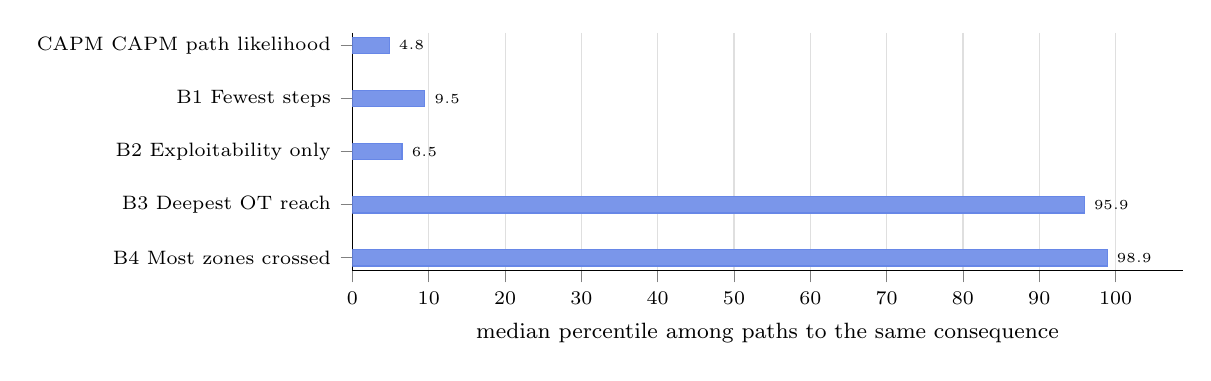
\begin{tikzpicture}
\begin{axis}[
    xbar, width=\linewidth, height=4.6cm,
    xlabel={median percentile among paths to the same consequence},
    xmin=0, enlarge y limits=0.06,
    ytick={0,1,2,3,4}, yticklabels={{CAPM CAPM path likelihood},{B1 Fewest steps},{B2 Exploitability only},{B3 Deepest OT reach},{B4 Most zones crossed}},
    y dir=reverse, ticklabel style={font=\scriptsize},
    label style={font=\footnotesize},
    nodes near coords, nodes near coords style={font=\tiny},
    every node near coord/.append style={/pgf/number format/fixed,
        /pgf/number format/precision=3},
    xmajorgrids, grid style={gray!25}, axis lines*=left,
    bar width=6pt, tick align=outside,
]
\addplot[fill=RoyalBlue!70, draw=RoyalBlue!80] coordinates {
        (4.800000,0)
        (9.500000,1)
        (6.500000,2)
        (95.900000,3)
        (98.900000,4)
};
\end{axis}
\end{tikzpicture}}
\caption{Median percentile of the corpus incidents under each prioritisation (lower is better). The segmentation- and depth-centric heuristics rank the routes that actually occurred near the bottom of their lists.}
\label{fig:baselines}
\end{figure}
